\chapter*{Dodatak: Prikaz aktivnosti grupe}
		\addcontentsline{toc}{chapter}{Dodatak: Prikaz aktivnosti grupe}
		
		\section*{Dnevnik sastajanja}
		
		%\textbf{\textit{Kontinuirano osvježavanje}}\\
		
		% \textit{U ovom dijelu potrebno je redovito osvježavati dnevnik sastajanja prema predlošku.}
		
		\begin{packed_enum}
			\item  sastanak
			
			\item[] \begin{packed_item}
				\item Datum: 14. listopada 2022
				\item Prisustvovali: D.Kiramarios, D.Kovačević, K.Tomičić, D.Jambrović, K.Orešković, K.Kijac, S.Barac
				\item Teme sastanka:
				\begin{packed_item}
					\item  raspodjela uloga (podjela poslova na frontend, backend i razvoj dokumentacije)
					\item  rasprava o zadanoj temi
					\item  sakupljanje pitanja za prvi sastanak sa asistenticom
				\end{packed_item}
			\end{packed_item}
			
			\item  sastanak
			\item[] \begin{packed_item}
				\item Datum: 20. listopada 2022
				\item Prisustvovali: D.Kiramarios, D.Kovačević, K.Tomičić, D.Jambrović, K.Orešković, K.Kijac, S.Barac
				\item Teme sastanka:
				\begin{packed_item}
					\item  osnovni podaci o izvođenju projekta
					\item  postavljanje pitanja vezanih za implementaciju projekta asistentici tijekom prvih pola sata sastanka i sljedećih 20 min
				\end{packed_item}
			\end{packed_item}

			\item  sastanak
			\item[] \begin{packed_item}
				\item Datum: 20. listopada 2022
				\item Prisustvovali: D.Kiramarios, D.Kovačević, K.Tomičić, D.Jambrović, K.Orešković, K.Kijac, S.Barac
				\item Teme sastanka:
				\begin{packed_item}
					\item  detaljna analiza zadatka
					\item  planiranje raspodjele poslova tijekom sljedećeg tjedna vezanih za inicijalizaciju backenda, frontenda i dokumentacije
					\item  dogovor o korištenju Jire za bolje praćenje raspodjele poslova
				\end{packed_item}
			\end{packed_item}

			\eject

			\item  sastanak
			\item[] \begin{packed_item}
				\item Datum: 23. listopada 2022
				\item Prisustvovali: D.Kiramarios, D.Kovačević, K.Tomičić, D.Jambrović, K.Orešković, K.Kijac, S.Barac
				\item Teme sastanka:
				\begin{packed_item}
					\item  pregled predložene skice klijentske aplikacije (frontend)
					\item  pregled predložene sheme za bazu podataka (backend)
					\item  pregled obrazaca uporabe i UC dijagrama (dokumentacija)
					\item  zaključak: male promjene sheme baze i slanje na pregled asistentici
				\end{packed_item}
			\end{packed_item}

			\item  sastanak
			\item[] \begin{packed_item}
				\item Datum: 24. listopada 2022
				\item Prisustvovali: D.Kiramarios, K.Tomičić, S.Barac
				\item Teme sastanka:
				\begin{packed_item}
					\item  detaljna analiza prijedloga dizajna za klijentsku aplikaciju
					\item  male promjene dizajna za klijentsku aplikaciju
					\item  podjela posla na klijentskoj aplikaciji među prisutnima
				\end{packed_item}
			\end{packed_item}
			
		\end{packed_enum}
		
		\eject
		\section*{Tablica aktivnosti}
		
			%\textbf{\textit{Kontinuirano osvježavanje}}\\
			
			 \textit{Napomena: Doprinose u aktivnostima treba navesti u satima po članovima grupe po aktivnosti.}

			\begin{longtblr}[
					label=none,
				]{
					vlines,hlines,
					width = \textwidth,
					colspec={X[7, l]X[1, c]X[1, c]X[1, c]X[1, c]X[1, c]X[1, c]X[1, c]}, 
					vline{1} = {1}{text=\clap{}},
					hline{1} = {1}{text=\clap{}},
					rowhead = 1,
				} 
				& \rotatebox{90}{\textbf{Dario Kiramarios }}
				& \rotatebox{90}{\textbf{David Kovačević }}
				& \rotatebox{90}{\textbf{Krunoslav Tomičić }}
				& \rotatebox{90}{\textbf{Dominik Jambrović }}
				& \rotatebox{90}{\textbf{Krešo Orešković }} 
				& \rotatebox{90}{\textbf{Karla Kijac }} 
				& \rotatebox{90}{\textbf{Sven Barac }} \\  
				Upravljanje projektom 		& 4 & 3 & 3 & 3 & 3 & 3 & 3\\ 
				Opis projektnog zadatka 	&  &  &  &  &  &  & \\ 
				Funkcionalni zahtjevi       &  &  &  & 2 &  &  &  \\ 
				Opis pojedinih obrazaca 	&  &  &  & 5 &  &  &  \\ 
				Dijagram obrazaca 			&  &  &  & 5 &  & 5 &  \\ 
				Sekvencijski dijagrami 		&  &  &  &  &  &  &  \\ 
				Opis ostalih zahtjeva 		&  &  &  & 1 &  &  &  \\ 
				Arhitektura i dizajn sustava	 &  &  &  & 1 &  &  &  \\ 
				Baza podataka				&  &  &  & 2 &  &  &   \\ 
				Dijagram razreda 			&  &  &  &  &  &  &   \\ 
				Dijagram stanja				&  &  &  &  &  &  &  \\ 
				Dijagram aktivnosti 		&  &  &  &  &  &  &  \\ 
				Dijagram komponenti			&  &  &  &  &  &  &  \\ 
				Korištene tehnologije i alati 		&  &  &  &  &  &  &  \\ 
				Ispitivanje programskog rješenja 	&  &  &  &  &  &  &  \\ 
				Dijagram razmještaja			&  &  &  &  &  &  &  \\ 
				Upute za puštanje u pogon 		&  &  &  &  &  &  &  \\  
				Dnevnik sastajanja 			&  &  &  &  &  &  &  \\ 
				Zaključak i budući rad 		&  &  &  &  &  &  &  \\  
				Popis literature 			&  &  &  &  &  &  &  \\  
				\hline
				\textit{Front end} 				& 4 &  & 3 &  &  &  & 3 \\  
				\textit{Izrada baze podataka} 		 			&  & 2 &  &  & 2 &  & \\  
				\textit{Spajanje s bazom podataka} 				&  &  &  &  &  &  &  \\ 
				\textit{Back end} 							&  &  &  &  &  &  &  \\  
				\textit{Popravak dokumentacije}			&  &  &  & 3 &  &  &  \\  
			\end{longtblr}
					
					
		\eject
		\section*{Dijagrami pregleda promjena}
		
		%\textbf{\textit{dio 2. revizije}}\\
		
		%unos slike
		\begin{figure}[H]
			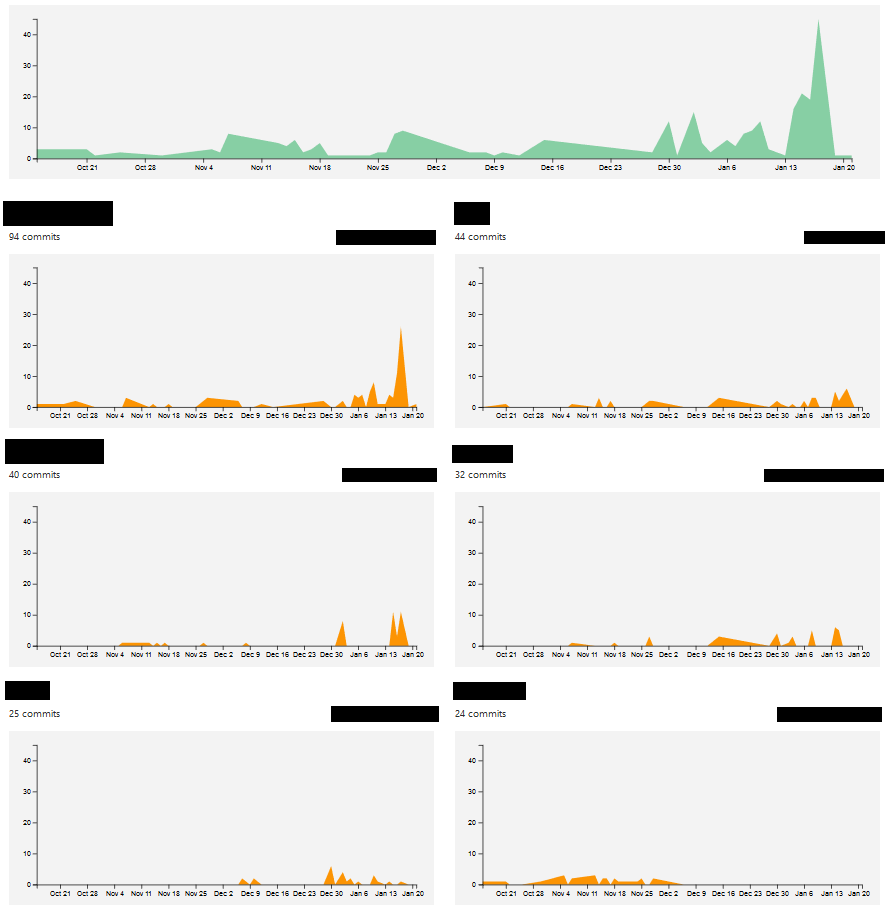
\includegraphics[scale=0.4]{slike/aktivnost.PNG}
			\centering
			\caption{Primjer slike s potpisom}
			\label{fig:promjene}
		\end{figure}